\documentclass{article}


\usepackage[margin=1.5cm, includefoot, footskip=30pt]{geometry}
\usepackage{amsmath}
\usepackage{amsthm}
\usepackage{booktabs}
\usepackage[sort]{cite}
\usepackage{caption}

\usepackage{tikz}
\usetikzlibrary{arrows.meta,positioning,calc,shadows.blur,fit,shapes.geometric}


\newtheorem{proposition}{Proposition}

\title{Hurt People Hurt People}
\author{M Harper and V Knight}
\date{\today}

\begin{document}

\maketitle

\abstract{

Adverse childhood experiences are strongly associated with lifelong health,
social, and economic outcomes, and increasing evidence suggests that their
effects may propagate across generations. While empirical studies document the
prevalence, transmission, and consequences of trauma, there is currently no
unified framework linking these individual-level mechanisms to population-level
dynamics. Here we combine a minimal analytical model with a data-informed
simulation model to study the long-term evolution of trauma prevalence. The
analytical model yields a closed-form threshold determining when trauma becomes
self-sustaining, while the simulation model incorporates heterogeneous exposure
levels and empirically grounded transmission patterns. The models show how
demographic processes, intergenerational transmission, and recovery interact to
produce stable endemic trauma levels or long-run decline, and establish the
conditions under which interventions can eliminate endemic prevalence.

}

\section{Introduction}

Adverse childhood experiences (ACEs) are widely recognised as major
determinants of lifelong health, social, and economic outcomes. The original
ACE study demonstrated strong associations between early adversity and a range
of adult disease risks \cite{felitti1998relationship}. Subsequent work has
shown that exposure to multiple forms of adversity is common across populations
\cite{joshi2021prevalence}. Meta-analytic evidence further indicates that
cumulative childhood adversity is strongly associated with both physical and
mental health outcomes throughout the life course
\cite{hughes2017effect}, with recent estimates suggesting that childhood
maltreatment alone may account for a substantial fraction of global mental
health burden \cite{grummitt2024burden}.

Trauma may also propagate across generations. Intergenerational transmission of
adversity has been documented across a range of social and developmental
contexts \cite{madigan2019intergenerational,schickedanz2021intergenerational},
and proposed mechanisms include behavioural pathways, socioeconomic
constraints, and biological processes such as epigenetic regulation
\cite{yehuda2016intergenerational}. Developmental research further emphasises
that early adversity can shape long-term stress responses and behavioural
trajectories \cite{shonkoff2012lifelong}, while resilience and recovery
processes can mitigate these effects under favourable conditions
\cite{masten2014ordinary,skolnick2023association}.

Exposure to harsh or unpredictable environments has been linked to accelerated
life-history strategies and earlier reproductive timing \cite{ellis2009fundamental},
and empirical studies have found associations between childhood adversity and
fertility patterns \cite{williams2019adverse}. Population prevalence is therefore
shaped by the interplay between transmission, demographic processes, and recovery.

No theoretical framework yet links these mechanisms to the long-term population
dynamics of trauma. Existing studies focus either on individual outcomes---documenting
associations between ACE exposure and adult health risk
\cite{felitti1998relationship}, synthesising dose--response relationships
\cite{hughes2017effect}, or characterising developmental consequences of early
toxic stress \cite{shonkoff2012lifelong}---or on statistical correlations across
cohorts, such as ACE prevalence estimates \cite{joshi2021prevalence} or
intergenerational transmission rates \cite{madigan2019intergenerational}.
Neither approach addresses how trauma prevalence evolves over long time horizons
or responds to structural interventions. Population modelling has proven useful
for linking demographic processes to long-run outcomes \cite{caswell2001matrix},
but has not been applied to trauma dynamics.

We develop a minimal analytical model that captures the essential mechanisms
required for trauma to persist or decline in a population. This model isolates
the roles of differential reproductive outcomes, intergenerational transmission,
and healing, and yields explicit threshold conditions for self-sustaining trauma
prevalence. We complement this with a data-informed simulation model
incorporating heterogeneous exposure levels and empirically grounded
transmission probabilities, which we use to explore how realistic distributions
of adversity shape long-run population outcomes.

Throughout this work \emph{adversity state} refers to an individual's level of
cumulative ACE exposure, not to any single event. Within a generation,
individuals move between lower and higher adversity states through exposure or
healing; across generations, adversity propagates via behavioural, socioeconomic,
and biological pathways. These mechanisms are illustrated in
Figure~\ref{fig:framework-overview}.

\begin{figure}[!hbtp]
\centering
    
\includegraphics[width=\textwidth]{./figures/figure_1/main.pdf}
\caption{\textbf{Core model structure and simulation algorithm.}
\textbf{(A)} Individuals occupy one of two adversity states, \(S\) (lower adversity) or \(T\)
(higher adversity), shown for two successive generations.
Within each generation, individuals transition from \(S\) to \(T\) with probability
\(p\) (exposure) and from \(T\) to \(S\) with probability \(q\) (healing).
Across generations, \(T\)-state individuals reproduce at rate \(\alpha f_S\)
relative to the baseline fertility \(f_S\) of \(S\)-state individuals (\(\alpha>1\)),
reflecting empirically observed associations between adversity and accelerated
life-history strategies.
Adversity propagates intergenerationally via behavioural, socioeconomic, and
biological pathways.
The product \(\alpha(1-q)\) acts as a demographic analogue of \(R_0\): endemic
trauma persists whenever \(\alpha(1-q)>1\).
\textbf{(B)} Flowchart of the individual-based simulation.
At each annual step the three processes act sequentially on every member of
the population denoted as \(\mathcal{P}_t\).
\emph{Reproduction}: surviving females may give birth with probability
\(b(a,k)\), which combines a tempo effect---shifting the baseline schedule
earlier by \(\tau\) years per ACE via effective age \(\tilde{a}=a-\tau k\)---and
a quantum effect---scaling the shifted probability by \(\alpha\) for individuals
with \(k\geq 1\) ACEs.
Each newborn is assigned a sex \(s'\) drawn from a Bernoulli with parameter
\(p_{\mathrm{m}}\) and an ACE count \(k'\) drawn from the empirical
intergenerational conditional distribution \(\Pr(k'\mid k)\).
\emph{ACE adjustment}: a surviving child (\(a<18\)) acquires one additional
ACE with probability \(p\) (trauma exposure); a surviving adult (\(a\geq 18\))
loses one ACE with probability \(q\) (healing).
\emph{Mortality}: each individual dies independently with the age- and
sex-specific probability \(\mu(s,a)\) taken from UN life tables; those who
die are excluded from \(\mathcal{P}_{t+1}\).
All survivors (with age incremented by one and ACE count updated) and all
newborns are collected into \(\mathcal{P}_{t+1}\).}
\label{fig:framework-overview}
\end{figure}

\section{Methods}

\subsection{Analytical model}

Individuals are assumed to be either traumatised or not, so the
population state is \(x=(x_T,x_S)\), where \(x_T\) denotes the proportion of
traumatised individuals and \(x_S=1-x_T\) the remainder.

Let \(f_T\) and \(f_S\) denote the fitness of the respective subpopulations.
Consistent with evidence linking adversity to accelerated life-history
strategies and elevated fertility, we set \(f_T=\alpha f_S\) with \(\alpha>1\)
\cite{ellis2009fundamental,williams2019adverse}.

We allow both the introduction of new trauma and the possibility of recovery
\cite{yehuda2016intergenerational,skolnick2023association}, modelled through
two parameters:

\begin{itemize}
    \item \(p\): probability that a non-traumatised individual becomes
    traumatised,
    \item \(q\): probability that a traumatised individual recovers.
\end{itemize}

Together, \(\alpha\), \(p\), and \(q\) determine the balance between
transmission, recovery, and differential reproduction, and hence whether trauma
prevalence grows, declines, or stabilises over time (Fig.~\ref{fig:trauma-dynamics}A).

\begin{figure}[!hbtp]
    \centering
        
\includegraphics[width=\textwidth]{./figures/figure_2/main.pdf}
    \caption{\textbf{Dynamics of trauma prevalence across mechanisms and parameters.}
\textbf{A}, Time evolution of the traumatised proportion \(x_T(t)\) under varying
exposure (\(p\)) and healing (\(q\)) regimes. Trajectories from high and low initial
conditions converge to the equilibrium level \(x^*\) (dotted line), illustrating
how persistent exposure or recovery processes determine long-run prevalence.
\textbf{B}, Analytical structure of the update map.
Top: net growth function \(\Delta(x_T)=x'_T-x_T\) for several values of the
relative reproductive multiplier \(\alpha\), showing how equilibrium number and
stability change with demographic amplification.
Bottom: phase portrait for a representative parameter set, with arrows
indicating the direction of population change.
\textbf{C}, Parameter landscape for the invasion regime (\(p=0\)).
The coloured surface shows the endemic equilibrium level \(x^*\) as a function of
\(\alpha\) and healing probability \(q\). The curve \(q=1-\frac{1}{\alpha}\) separates
parameter combinations for which trauma necessarily declines from those where it
can persist endemically.
\textbf{D}, Corresponding landscape with positive background exposure (\(p=0.05\)).
Introducing a non-zero exposure rate eliminates the trauma-free state, raising
\(x^*\) across the entire parameter space and shifting the effective persistence
boundary upward.}
    \label{fig:trauma-dynamics}
\end{figure}

The population evolves according to the discrete replicator--mutation dynamic
\cite{imhof2005evolutionary,nowak2006evolutionary},
\[
x_i'=\sum_{j\in\{T,S\}}\frac{x_j f_j Q_{ji}}{\bar f},
\qquad i\in\{T,S\},
\]
with mutation matrix
\[
Q=
\begin{pmatrix}
1-q & q \\
p   & 1-p
\end{pmatrix}.
\]
The resulting update rule for the traumatised proportion is
\[
x_T'
=\frac{x_T f_T(1-q)+x_S f_S p}{\bar f}.
\]

To assess persistence, consider the growth factor
\(\kappa_T=x_T'/x_T\).
Substituting \(f_T=\alpha f_S\) and \(x_S=1-x_T\) yields
\[
\kappa_T
=\frac{1}{x_T}
\frac{x_T\bigl(\alpha(1-q)-p\bigr)+p}{x_T(\alpha-1)+1}.
\]
Values \(\kappa_T>1\) imply growth of the traumatised subpopulation,
while \(\kappa_T<1\) imply decline, reflecting the standard 
growth criterion used in evolutionary dynamics
\cite{nowak2006evolutionary,hofbauer1998evolutionary}.

Interior equilibria satisfy \(x_T'=x_T\), leading to the quadratic

\[
(\alpha-1)x_T^2+(1+p-\alpha+\alpha q)x_T-p=0,
\]

Because the constant term equals \(-p<0\) while evaluation at
\(x_T=1\) gives \(\alpha q\ge0\), continuity guarantees a root in
\((0,1)\) whenever \(p,q>0\).
This root defines the endemic level \(x_T^*\), showing that any
persistent introduction of trauma produces a stable long-run
prevalence (Fig.~\ref{fig:trauma-dynamics}A).

When no new trauma is introduced (\(p=0\)), persistence depends on invasion
from rarity. Taking the limit \(x_T\to0\) gives
\[
\lim_{x_T\to0}\kappa_T=\alpha(1-q),
\]
so trauma spreads from low prevalence precisely when
\[
\alpha(1-q)>1
\qquad\Longleftrightarrow\qquad
q<1-\frac{1}{\alpha}.
\]
This condition acts as a demographic threshold separating extinction from
endemic persistence, shown in Fig.~\ref{fig:trauma-dynamics}C.

\medskip

Long-run trauma prevalence is therefore governed by the balance between
transmission, recovery, and demographic reinforcement. A sufficient reproductive
advantage can sustain trauma across generations even without continual exposure,
and recovery must cross a critical threshold to eliminate it. The system behaves,
in this respect, like an infectious agent with a demographic amplification
mechanism.

Figure~\ref{fig:trauma-dynamics}B--C summarises the equilibrium structure.
The next section embeds these mechanisms in a data-informed simulation that
adds demographic stochasticity, age structure, and empirically grounded
parameterisation.

\section{Individual-based simulation model}

To explore how stochasticity, finite-population effects, and demographic
heterogeneity modify the analytical predictions, we built an individual-based
simulation of the same mechanisms.

\subsection*{Individual state and population dynamics}

Each individual is characterised by a triple \((s, a, k)\) denoting sex
\(s \in \{\text{M}, \text{F}\}\), integer age \(a \geq 0\), and ACE count
\(k \in \{0, 1, \dots, 8\}\).  The population at time \(t\) is the multiset
\(\mathcal{P}_t = \{(s_i, a_i, k_i)\}_{i=1}^{N_t}\), where \(N_t\) is the
(stochastic) population size.  The model evolves in discrete yearly steps; in
each step three processes act sequentially on every individual: mortality,
reproduction, and within-life ACE adjustment.

\subsection*{Mortality}

Each individual \((s, a, k)\) dies in year \(t\) with probability \(\mu(s, a)\),
drawn from age- and sex-specific life-table values based on UN World Population
Prospects data \cite{un_wpp_mortality}.  Mortality is assumed independent of
ACE count, so demographic selection operates exclusively through fertility.

\subsection*{Fertility and ACE transmission}

Reproduction is restricted to surviving females.  The baseline probability of a
birth in a given year for a female of age \(a\) is \(b_0(a)\), taken from UN
age-specific fertility schedules \cite{un_wpp_fertility}.  Two empirically
motivated mechanisms modify this baseline for ACE-exposed individuals.

\paragraph{Tempo effect (earlier reproductive timing).}
Consistent with evidence that adversity is associated with accelerated
life-history strategies and earlier age at first birth
\cite{williams2019adverse}, the fertility schedule is shifted earlier in
proportion to ACE exposure.  Specifically, a female with \(k \geq 1\) ACEs
evaluates her birth probability at an effective age
\[
    \tilde{a} = a - \tau k,
\]
where \(\tau > 0\) is the tempo parameter (years of schedule shift per ACE).
Empirical estimates suggest \(\tau \approx 3\)
\cite{williams2019adverse}, which is used here.
This implements a purely timing adjustment: completed fertility is unaffected
in the absence of the quantum mechanism described below.

\paragraph{Quantum effect (differential reproductive intensity).}
Conditional on effective age \(\tilde{a}\), the birth probability of a female
with \(k \geq 1\) ACEs is scaled by a multiplicative factor \(\alpha > 1\):
\[
    b(a, k) =
    \begin{cases}
        b_0(\tilde{a})          & \text{if } k = 0, \\
        \min\!\bigl(1,\, \alpha\, b_0(\tilde{a})\bigr) & \text{if } k \geq 1.
    \end{cases}
\]
Under a coarse-grained binary classification (ACE-free versus ACE-exposed),
this corresponds directly to the relative fitness parameter of the analytical
model, in which \(f_T = \alpha f_S\).  The simulation therefore embeds the
replicator structure of the analytical model within an age-structured,
stochastic demographic framework.

\paragraph{Intergenerational ACE transmission.}
The ACE count of each newborn is drawn from an empirically estimated
conditional distribution \(\Pr(k_{\text{child}} \mid k_{\text{mother}})\), based
on reported intergenerational ACE correlations \cite{intergenerational_aces}.
Denoting the four maternal exposure categories as \(\{0, 1, 2\text{--}3,
\geq 4\}\), the conditional probabilities are summarised in
Table~\ref{tab:intergenerational}.  Offspring ACE counts in the range
\(\{2, 3\}\) and \(\{4, \dots, 8\}\) are distributed uniformly within their
respective groups.  This mechanism allows adversity to propagate across
generations in the absence of ongoing environmental shocks, providing the
simulation analogue of the transmission parameter \(p\) in the analytical model.

\begin{table}[!htbp]
    \centering
    \caption{Conditional probabilities \(\Pr(k_{\text{child}} \mid k_{\text{mother}})\)
    for offspring ACE category given maternal ACE category, expressed as percentages
    with 95\% confidence intervals. Source: \cite{schickedanz2021intergenerational}.}
    \label{tab:intergenerational}
    \begin{tabular}{lcccc}
        \toprule
        & \multicolumn{4}{c}{Maternal ACE category} \\
        \cmidrule(lr){2-5}
        Child ACE category & 0 & 1 & 2--3 & \(\geq 4\) \\
        \midrule
        0       & 42.6 (38.4--46.7) & 37.8 (32.4--43.1) & 30.4 (24.7--36.1) & 25.1 (16.2--34.0) \\
        1       & 25.8 (21.9--29.6) & 29.7 (23.9--35.5) & 28.4 (22.2--34.7) & 23.2 (14.1--32.2) \\
        2--3    & 25.8 (21.9--29.7) & 21.5 (16.3--26.7) & 21.3 (15.7--26.8) & 23.8 (15.6--32.0) \\
        \(\geq 4\) & 5.8 (4.0--7.7)  & 11.0 (6.3--15.6)  & 19.9 (13.7--26.1) & 27.9 (18.9--36.9) \\
        \bottomrule
    \end{tabular}
\end{table}

\subsection*{Within-life ACE dynamics}

ACE counts may change within a lifetime through two complementary processes
that correspond directly to the analytical parameters \(p\) and \(q\).

\begin{itemize}
    \item \emph{Trauma exposure} (\(p\)): a child aged \(a < 18\) acquires one
    additional ACE with probability \(p\) per year, subject to the ceiling
    \(k \leq 8\).  This represents environmental and social transmission of
    adversity during the developmental window.
    \item \emph{Healing} (\(q\)): an adult aged \(a \geq 18\) reduces their ACE
    count by one with probability \(q\) per year, subject to the floor \(k \geq 0\).
    This represents recovery processes including therapeutic intervention,
    social support, and self-forgiveness
    \cite{skolnick2023association,trauma_recovery_processes}.
\end{itemize}

The net annual change in ACE count for individual \(i\) is therefore
\[
    \Delta k_i =
    \begin{cases}
        +1 & \text{if } a_i < 18 \text{ and } U_i < p, \\
        -1 & \text{if } a_i \geq 18 \text{ and } U_i < q, \\
        0  & \text{otherwise,}
    \end{cases}
\]
where \(U_i \sim \mathrm{Uniform}(0,1)\) is drawn independently each year.
\(p\) and \(q\) play the same roles in the simulation as in the analytical
model: \(p\) governs the rate of acquiring adversity and \(q\) the recovery rate.

\subsection*{Initial conditions}

Simulations are initialised from a population pyramid based on UK Office for
National Statistics census data \cite{ons_population_pyramid}, from which ages
and sexes are sampled according to empirical proportions.  Initial ACE counts
are drawn from sex-stratified prevalence distributions reported in the Canadian
Longitudinal Study on Aging \cite{joshi2021prevalence}.

\subsection*{Relationship to the analytical model}

The simulation preserves the core dynamical structure---\(\alpha\), \(p\), and
\(q\) enter with the same meanings as in the replicator--mutation model---but
replaces the mean-field assumption with explicit demographic stochasticity and
age structure, and the binary ACE state with a discrete count on
\(\{0, \dots, 8\}\).  In the limit of large population size and binary
aggregation of the ACE count, the simulation dynamics converge to the analytical
predictions; departures reflect stochasticity and heterogeneity.

To identify the boundary between high- and low-adversity parameter regimes in
the simulation output we applied \(k\)-means clustering (\(k=2\)) to the log-transformed mean ACE
surface; full details of this procedure are given in
Supplementary Information~\ref{si:kmeans}.

Figure~\ref{fig:population-dynamics} illustrates the baseline demographic
behaviour of the simulation across six parameter combinations
(\(q \in \{0.00, 0.01, 0.05\}\), \(\alpha \in \{1.05, 1.35\}\), no background
exposure): population size and mean age converge to stable levels within a
few decades across all combinations (panels A--B), and the empirical
survivorship curves closely match the theoretical life-table predictions
irrespective of ACE parameters, confirming that mortality is
ACE-independent (panel C).  Population age pyramids at 50-year intervals
(panels D--H) show the transition from the initial UK age structure to the
long-run steady-state shape for a representative parameter set
(\(q = 0.05\), \(\alpha = 1.35\), no background exposure).

\begin{figure}[!hbtp]
    \centering
        
\includegraphics[width=\textwidth]{./figures/figure_3/main.pdf}
    \caption{\textbf{Population-level demographic dynamics of the simulation.}
Results shown for six parameter combinations (\(q \in \{0.00, 0.01, 0.05\}\),
\(\alpha \in \{1.05, 1.35\}\), no background exposure) to demonstrate that
the demographic dynamics are robust across the parameter space explored.
\textbf{A}, Trajectories of total population size over 200 years (median
\(\pm\) IQR across replicates, one line per parameter combination).
\textbf{B}, Mean age of the population over time, with the same summary.
\textbf{C}, Empirical period survivorship \(l(x) = N(x)/N(0)\) computed from
simulation snapshots after year 100.
One pair of median lines (male and female sharing the same colour and line
style) is shown per parameter combination.
The grey band shows the pooled inter-quartile range across all parameter
combinations and replicates.
Dark grey lines show the theoretical survivorship curves derived directly
from the UN life-table probabilities (solid: male; dashed: female).
The close agreement across all parameter combinations confirms that the
simulated age structure is consistent with the embedded mortality schedule
and is insensitive to the ACE transmission parameters, as expected given
that mortality is modelled as ACE-independent.
\textbf{D--H}, Population age pyramids (median counts across replicates) at
years 0, 50, 100, 150, and 200 for the representative parameter set
(\(q = 0.05\), \(\alpha = 1.35\), no background exposure), showing the
transition from the initial UK census age structure to the long-run
steady-state shape imposed by the empirical fertility and mortality schedules.}
    \label{fig:population-dynamics}
\end{figure}

\begin{figure}[!hbtp]
    \centering
        
\includegraphics[width=\textwidth]{./figures/figure_4/main.pdf}
    \caption{\textbf{Simulation outcomes across parameter regimes (mean ACE count).}
Panels are arranged in three rows and two columns; the left column shows
results without background trauma exposure (\(p = 0\)) and the right column
with positive background exposure (\(p = 0.2\)).
\textbf{A--B}, Time trajectories of mean ACEs per person for six combinations
of healing probability \(q\) and reproductive multiplier \(\alpha\), shown as
median \(\pm\) IQR across simulation replicates.  The dashed vertical line marks
the end of the 100-year warm-up period.
\textbf{C--D}, Mean \(\pm\) SD of mean ACE count as a function of \(\alpha\),
with one curve per healing probability.  Higher \(\alpha\) and lower \(q\)
consistently raise long-run adversity levels, with the effect amplified under
positive background exposure.
\textbf{E--F}, Heatmaps of the time-averaged mean ACE count in the
\((q, \alpha)\) parameter plane, shown on a \(\log(1 + \cdot)\)
scale.  The dashed red contour marks the \(k\)-means threshold separating high- and
low-adversity regimes; the linear fit \(q^* = m\alpha + c\) (shown in each
panel title) recovers a boundary consistent with the analytical condition
\(q > 1 - \alpha^{-1}\).  Corresponding results for the proportion-traumatised
metric are shown in Fig.~\ref{fig:simulation-outcomes-si}.}
    \label{fig:simulation-outcomes}
\end{figure}

\section{Discussion}


Our central result is a closed-form threshold,
\(q < 1 - 1/\alpha\), separating parameter regimes in which trauma
necessarily declines from those in which it persists endemically.
Any positive background exposure (\(p > 0\)) eliminates the trauma-free
equilibrium entirely: the quadratic fixed-point equation always admits an
interior root, so even a small rate of environmental adversity produces a
stable long-run prevalence.  The individual-based simulation corroborates these
analytical predictions; demographic stochasticity and age structure shift the effective boundary but do not
qualitatively alter the prediction.

The threshold condition \(\alpha(1-q) > 1\) is structurally analogous to the
basic reproduction number \(R_0\) in infectious-disease epidemiology
\cite{hofbauer1998evolutionary}, with the product \(\alpha(1-q)\) playing the
role of \(R_0\).  Unlike standard SIS/SIR frameworks, this system contains a demographic
amplification term: adversity is not merely transmitted but is reinforced by a
reproductive advantage that standard epidemic models lack.

The parameter \(\alpha > 1\) reflects observed associations between early
adversity and accelerated life-history strategies
\cite{ellis2009fundamental,williams2019adverse}.  This does not imply that
trauma is adaptive; it captures empirically documented tempo and quantum effects
on reproductive timing and intensity.  The tempo effect (earlier age at first birth) and the
quantum effect (elevated birth rates conditional on effective age) make
separable contributions to persistence, and the threshold condition provides a
way to quantify their joint role.  The empirical range of \(\alpha\) in
contemporary populations suggests that many settings may lie close to or above
the persistence threshold.

The simulation broadly corroborates the analytical predictions. Without
background exposure, mean ACE trajectories converge to moderate endemic levels
from a range of initial conditions (Fig.~\ref{fig:simulation-outcomes}A),
consistent with the stable interior equilibrium. Positive background exposure
raises the outcome substantially and widens variation across parameter
combinations (Fig.~\ref{fig:simulation-outcomes}B), confirming that even modest
environmental transmission eliminates the trauma-free state. The summary panels
(Fig.~\ref{fig:simulation-outcomes}C--D) show a consistent ordering: higher
\(\alpha\) and lower \(q\) raise long-run adversity, with the effect amplified
under positive background exposure. At \(q = 0.05\), mean ACE counts are
suppressed near zero at moderate \(\alpha\) when \(p = 0\), but only partially
attenuated when \(p > 0\). The heatmaps (Fig.~\ref{fig:simulation-outcomes}E--F)
show the transition is well approximated by a linear threshold
\(q^*(\alpha) = m\alpha + c\) (\(R^2 \geq 0.99\)). Fitted slopes are modest
without background exposure (\(m \approx 0.013\)) but roughly four-fold steeper
under positive background exposure (\(m \approx 0.042\)). The positive intercepts
(\(c \approx 0.025\)--\(0.168\)) imply a minimum healing requirement even as
\(\alpha \to 1\), consistent with any \(p > 0\) shifting the equilibrium
landscape upward. Results for the proportion-traumatised metric are qualitatively
identical (Fig.~\ref{fig:simulation-outcomes-si}). The threshold separating
suppression from persistence scales approximately linearly with \(\alpha\);
background exposure raises it, so addressing transmission and healing separately
is insufficient.

To drive the system below endemic persistence, \(q\) must exceed
\(1 - 1/\alpha\); any intervention that reduces \(\alpha\) simultaneously
lowers the required healing rate.  Interventions combining socioeconomic support
with expanded therapeutic access are therefore doubly effective, acting on both
factors in \(\alpha(1-q)\).  The empirical linear relationship
\(q^*(\alpha) = m\alpha + c\) implies that populations with higher \(\alpha\)
require proportionally more intensive recovery programmes.

Several limitations apply.  Both models simplify adversity: the analytical model
uses a binary state, the simulation a discrete count on \(\{0,\dots,8\}\), and
neither captures continuous severity or multi-domain ACE categorisations.
Mortality is ACE-independent, though emerging evidence links high ACE burden to
premature mortality, which would reduce the effective \(\alpha\) and lower the
persistence threshold.  No spatial or network structure is included, so local
clustering of adversity and peer transmission are not represented.  Finally,
\(\alpha\) and \(\tau\) were calibrated from UK and Canadian data; cross-cultural
variation remains unexplored.

Extensions could include multi-domain ACE severity, spatial and network
structure, and cross-national calibration of \(\alpha\).  The threshold condition
offers a direct basis for evaluating intervention cost-effectiveness.  The
framework gives population-level adversity science the same formal structure as
epidemic theory: a minimal model with an explicit persistence threshold.

\bibliographystyle{plain}
\bibliography{bibliography.bib}

\newpage
\appendix
\section*{Supplementary Information}
\addcontentsline{toc}{section}{Supplementary Information}

\subsection{Simulation outcomes: proportion-traumatised metric}
\label{si:prop-traumatised}

\begin{figure}[!htbp]
    \centering
        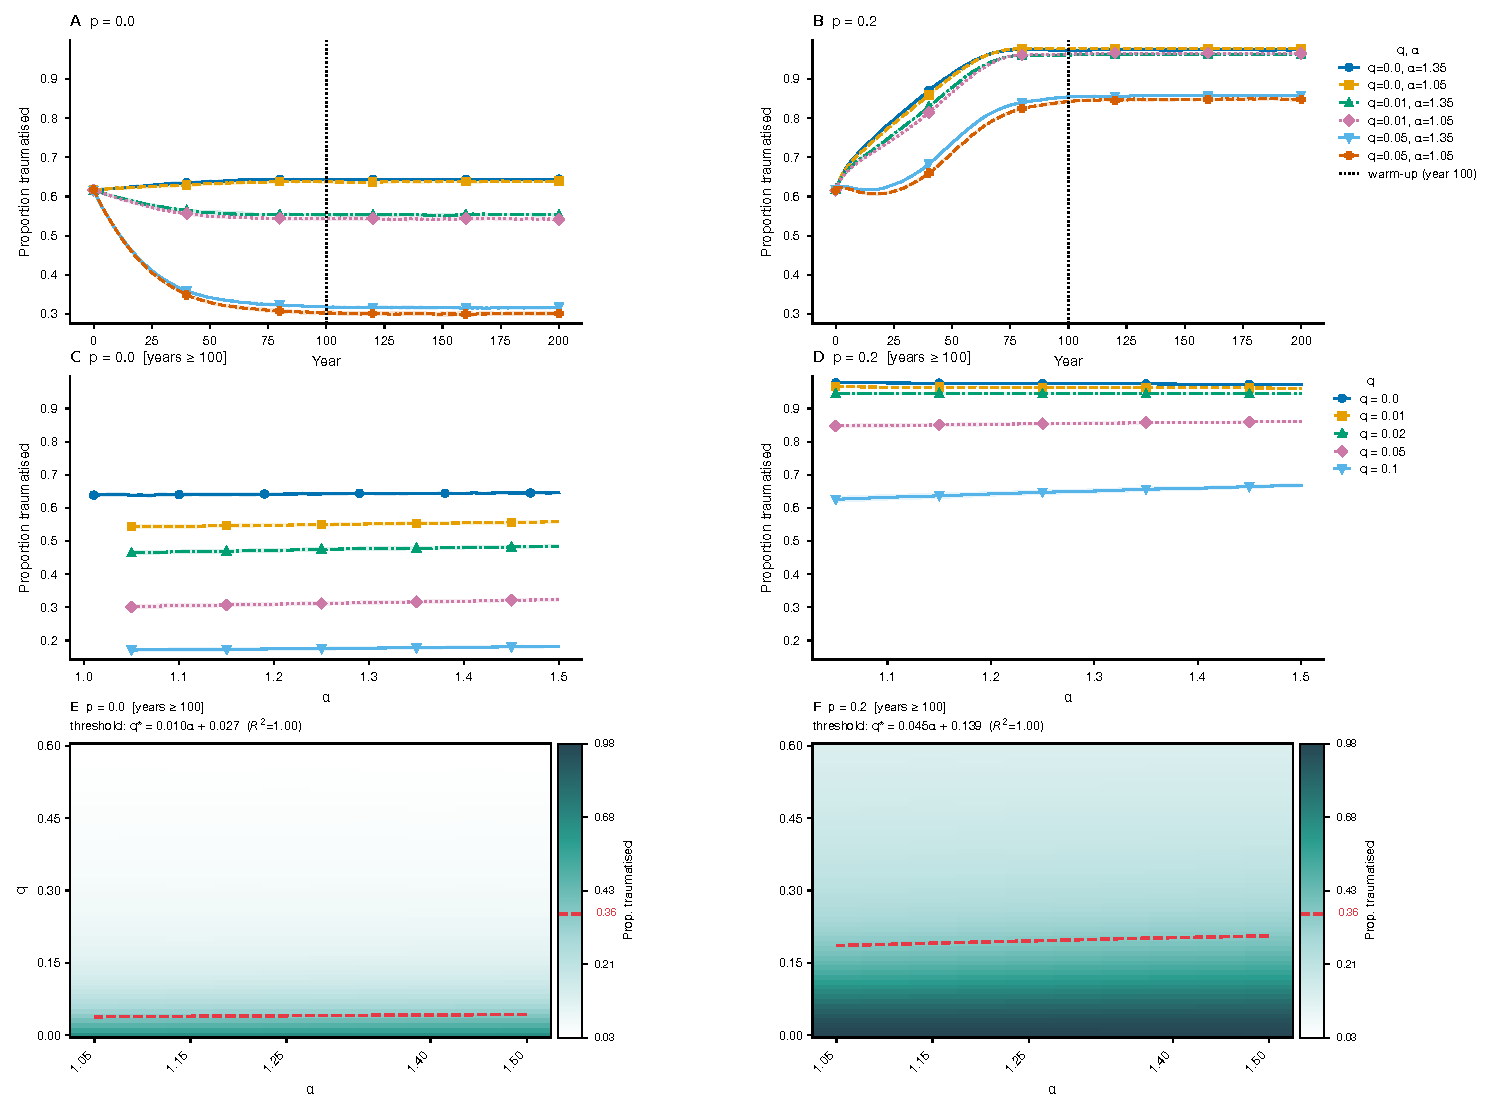
\includegraphics[width=\textwidth]{./figures/figure_4/si.pdf}
    \caption{\textbf{Simulation outcomes across parameter regimes (proportion traumatised).}
Layout mirrors Fig.~\ref{fig:simulation-outcomes}.  Left column: no background
trauma exposure (\(p = 0\)); right column: positive background exposure
(\(p = 0.2\)).
\textbf{A--B}, Time trajectories of the proportion of individuals with at least
one ACE for the same six parameter combinations as Fig.~\ref{fig:simulation-outcomes},
shown as median \(\pm\) IQR.
\textbf{C--D}, Mean \(\pm\) SD of proportion traumatised as a function of
\(\alpha\), one curve per healing probability.
\textbf{E--F}, Heatmaps of the time-averaged proportion traumatised in the
\((q, \alpha)\) parameter plane (\(\log(1+\cdot)\) scale).  The
dashed red contour marks the \(k\)-means threshold; the linear fit \(q^* = m\alpha + c\)
is consistent with the mean-ACE results in Fig.~\ref{fig:simulation-outcomes}E--F.}
    \label{fig:simulation-outcomes-si}
\end{figure}

\subsection{\(k\)-means threshold across all values of \(p\)}
\label{si:threshold-vs-p}

\begin{figure}[!htbp]
    \centering
        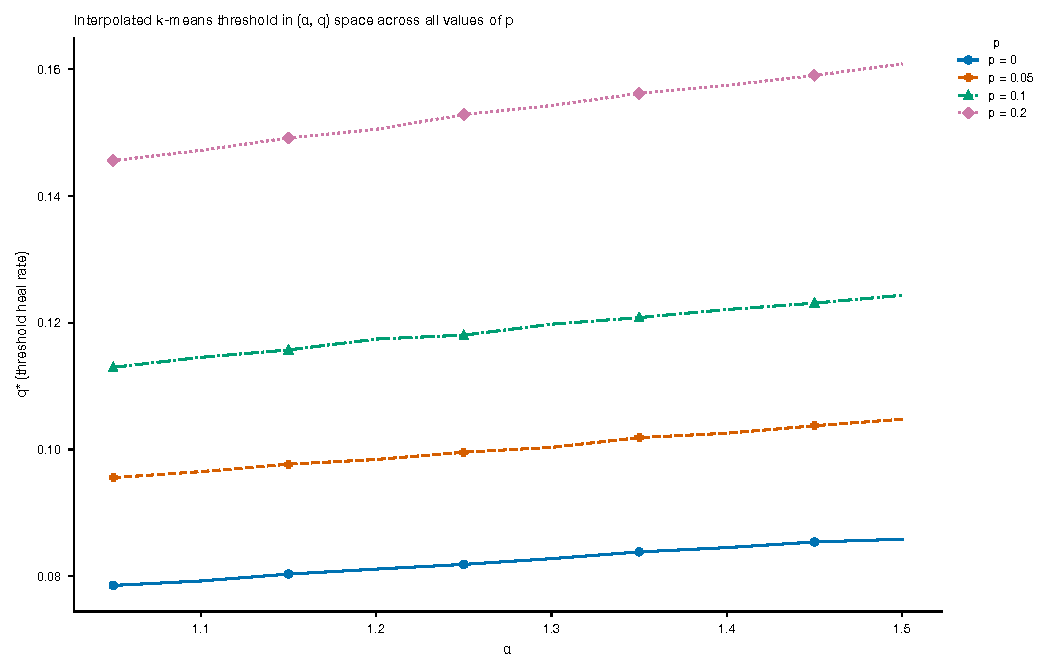
\includegraphics[width=0.75\textwidth]{./figures/figure_4/si_threshold.pdf}
    \caption{\textbf{\(k\)-means threshold contours across all values of \(p\).}
Each curve shows \(q^*(\alpha)\) for a single value of the background exposure probability \(p\)
(identified by colour, linestyle, and marker; see legend).
The threshold is computed for each \(p\) separately by \(k\)-means (\(k = 2\)) on the
\(\log(1+\cdot)\)-transformed mean ACE surface and located by linear interpolation along the \(q\)-axis.
Higher \(p\) shifts the threshold upward.}
    \label{fig:threshold-vs-p}
\end{figure}

\subsection{\(k\)-means threshold procedure}
\label{si:kmeans}

To identify the boundary between parameter regimes that sustain high and low
levels of adversity, we applied \(k\)-means clustering with \(k = 2\) \cite{lloyd1982least} to the
log-transformed mean ACE surface.
Let \(\bar{k}(q, \alpha)\) denote the mean ACE count averaged across all years
and simulation replicates at healing probability \(q\) and reproductive
multiplier \(\alpha\), and let
\(\ell(q, \alpha) = \log\bigl(1 + \bar{k}(q, \alpha)\bigr)\)
be its \(\log(1 + \cdot)\) transform, applied to compress the dynamic range
of the surface and to handle zero values stably.
\(k\)-means partitions the observed values of \(\ell\) into two clusters by
iteratively assigning each value to its nearest cluster centre and updating
centres to cluster means until convergence (initialised at the 25th and 75th
percentiles of \(\ell\)). The scalar threshold \(\ell^*\) is the midpoint
between the two converged cluster centres, and requires no user-specified cutoff.
The threshold defines a level set
\(\{(q, \alpha) : \ell(q, \alpha) = \ell^*\}\)
in the original parameter space, which we locate for each value of \(\alpha\)
by linear interpolation along the \(q\)-axis to obtain crossing points
\(q^*(\alpha)\).
Although the threshold is identified in log-space, the resulting boundary is
expressed in the untransformed coordinates \((q, \alpha)\), and is well
described by a linear relationship
\[
    q^*(\alpha) = m\alpha + c,
\]
recovered by ordinary least squares regression on the interpolated crossing
points (fits shown in panel titles; \(R^2 > 0.95\) in all cases).
This linear structure implies that the critical healing probability required to
suppress endemic adversity scales proportionally with the reproductive
multiplier \(\alpha\), consistent with the analytical threshold condition
\(q > 1 - \alpha^{-1}\) derived in Section~2 (Fig.~\ref{fig:simulation-outcomes}).
Fig.~\ref{fig:threshold-vs-p} shows the resulting threshold contours for every value of \(p\) in the data.

\end{document}
